\chapter{Fiducial region definition and optimization}
\label{app:fiducial_region}

The fiducial region must be chosen in such a way to be as close as possible to the selections applied in the analysis, in order to reduce the model dependece in the extrapolation step. That means that for optimizing the fiducial volume definition, the efficiency has to be maximized. Another parameter entering the game is the number of fake events, in other words the number of reconstructed events which do not belong to the fiducial phase space. This parameter should instead be as small as possible. Even if we have to observe the trend of these two quantities as a function of \pth, we can maximize the ratio between the overall efficiency and the overall fake rate as a proxy for establishing the ``goodness'' of the fiducial region.

Several different fiducial region definitions were tested and the results show that:
\begin{itemize}
\item {\bf of cut:} The fiducial region definition must include only the opposite flavor combination including one electron and one muon. If we include also the combinations involving $\tau$'s the efficiency falls down.
\item {\bf Lepton cut:} Since the resolution on lepton transverse momentum is good, there is no need to loosen the cuts related these variables, i.e. we can use the same cuts defined in the analysis selection ($\pt^{\ell,1}>20$\GeV, $\pt^{\ell,2}>10$\GeV).
\item {\bf Di-lepton \pt cut:} As stated in the previous point, there is no need to loosen this cut, so we kept the same value as the analysis selection, i.e. $\ptll>30$\GeV.
\item {\bf Di-lepton mass cut:} $\mll>12$\GeV as discussed before.
\item {\bf neutrino pair \pt cut:} Since the resolution on the measurement of the missing transverse energy is poor, the neutrino pair cut should not be included in the definition of the fiducial region, because it would increase the fake rate without increasing the efficiency, thus resulting in a lower ratio between overall efficiency and fake rate.
\item {\bf \mt cut:} Also the \mt cut that we have in the analysis selection, i.e. $\mt>60$\GeV, should be loosened or removed because it involves neutrinos and then increase the fake rate. We decided eventually to keep this cut, loosening it to 50\GeV, because in addition to increase the number of fake events, it increases the efficiency as well.
\end{itemize}

The fake rate and the efficiency as a function of \pth after the optimization discussed before are shown in figure \ref{fig:eff_fake_comp}. To obtain these plots the fiducial region was modified adding in sequence the various cuts and computing the efficiency and the fake rate each time. In that way we can asses the composition of those distributions.

\begin{figure}[htb]
\centering
\subfigure{
\includegraphics[width=0.5\textwidth]{images/eff_optimized.pdf}
}
\subfigure{
\includegraphics[width=0.5\textwidth]{images/fake_optimized.pdf}
}
\caption{Efficiency and fake rate as a function on Higgs transverse momentum. The plots correspond to the optimized fiducial region definition and show the effect of adding each of the mentioned cuts in sequence.}\label{fig:eff_fake_comp}
\end{figure}

The efficiency and fraction of fake events have been measured also as a function of the \MET and \mt cuts in the fiducial region. Since these two variables are correlated, the results are reported as two-dimensional histograms. In Fig.~\ref{fig:eff_fake_nom} are reported the efficiency and fraction of fake events for these two variables.

\begin{figure}[htb]
\centering
\subfigure{
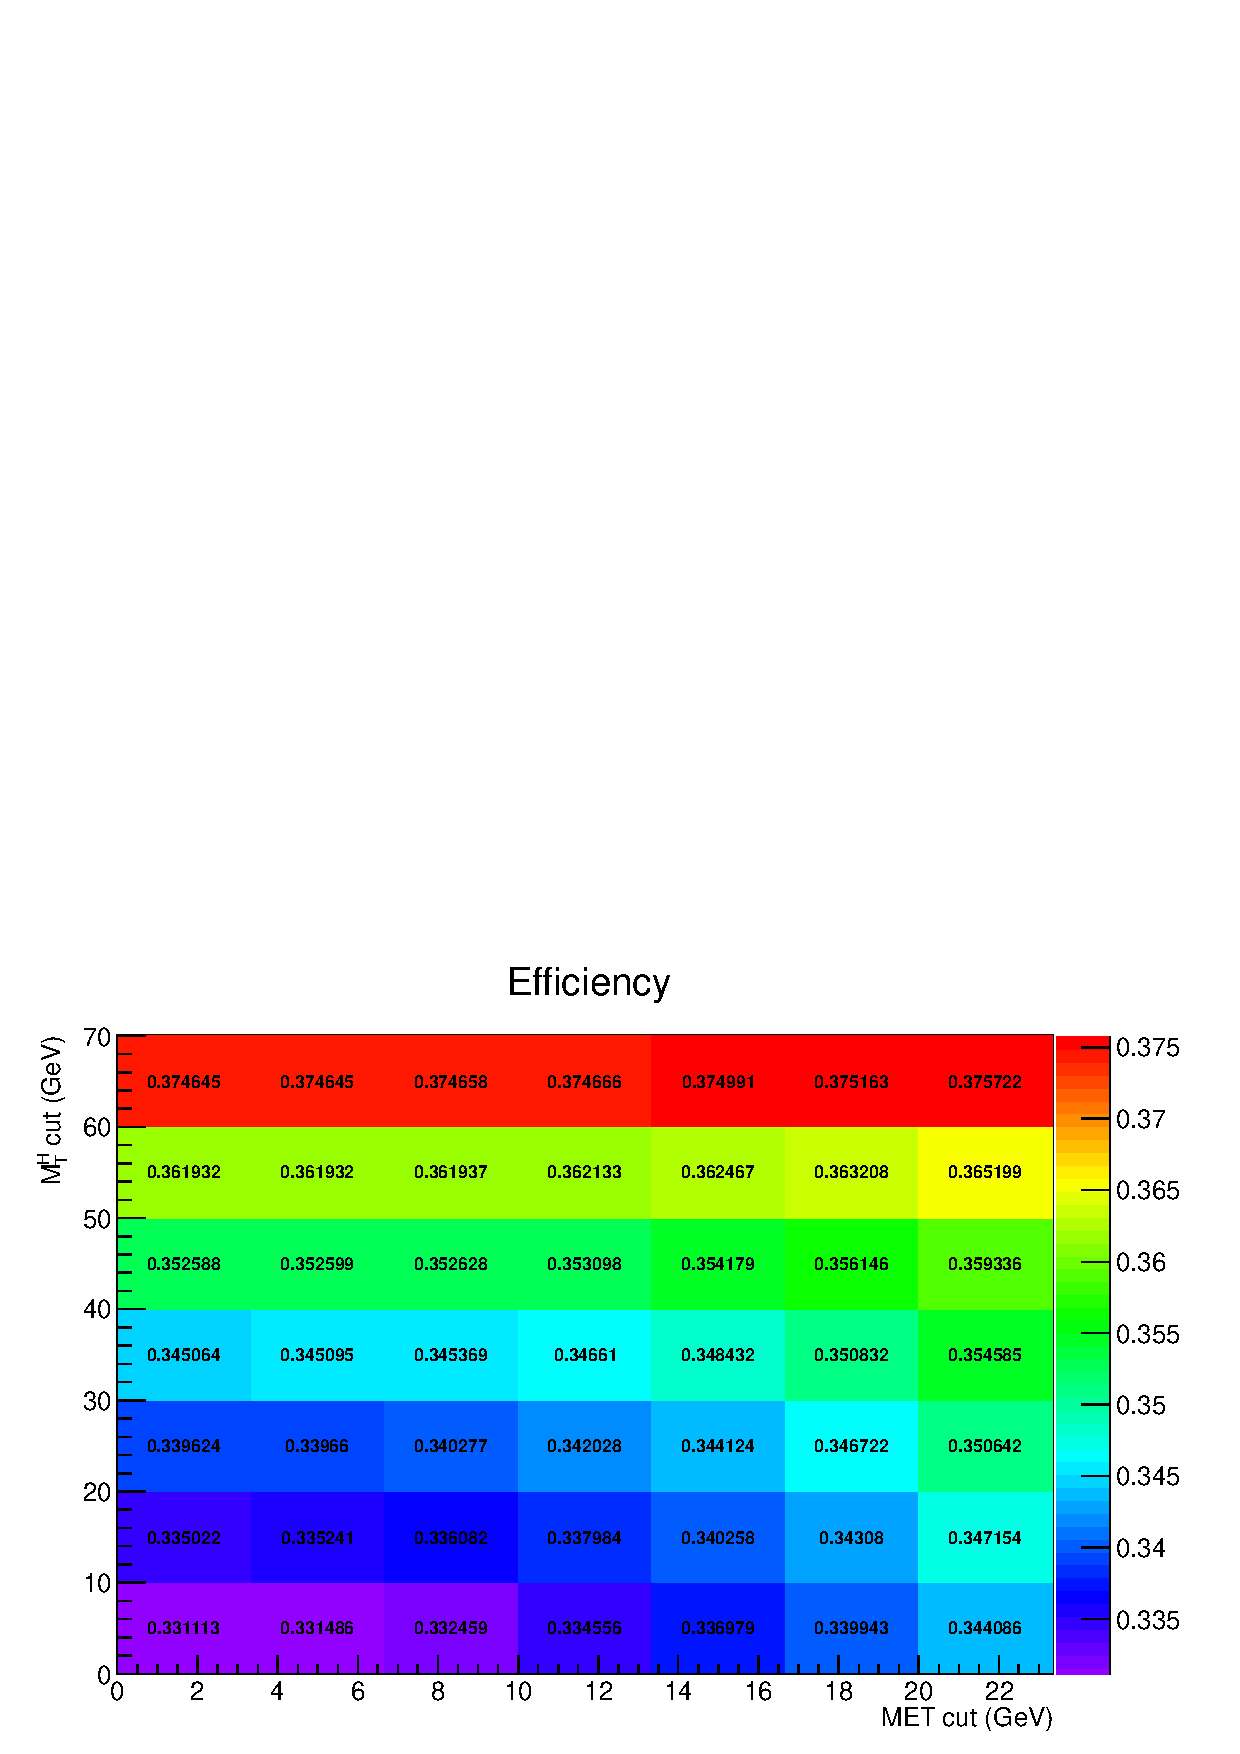
\includegraphics[width=0.5\textwidth]{images/met_mth_eff.pdf}
}
\subfigure{
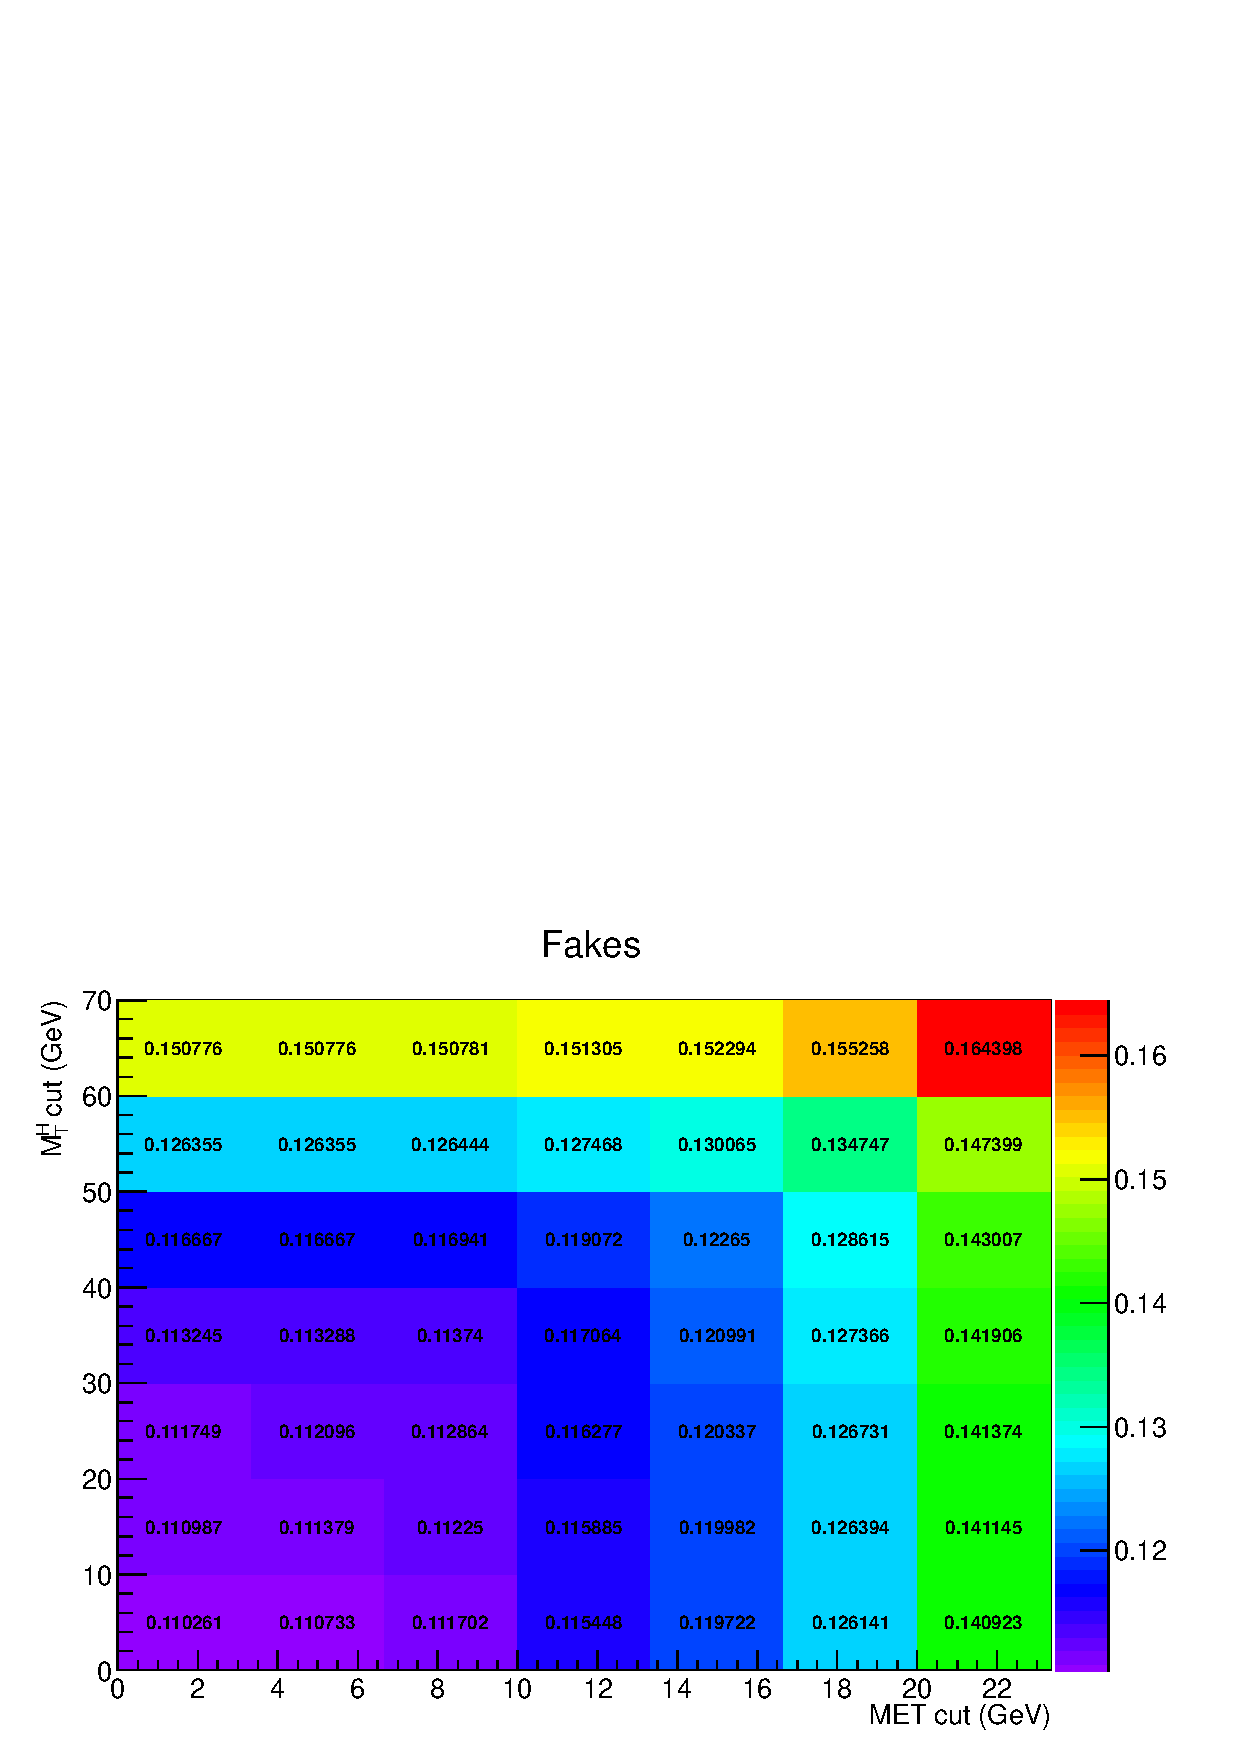
\includegraphics[width=0.5\textwidth]{images/met_mth_fake.pdf}
}
\caption{Efficiency and fake rate as a function of \MET and \mt cuts in the fiducial region.}\label{fig:eff_fake_nom}
\end{figure}

The criterion adopted to define the fiducial region is a tradeoff between having a large efficiency and a small fraction of fake events. Especially when looking at the low resolution variables, such as \MET and \mt, a suitable figure of merit has to be chosen for the estimation of the best cuts.  Several different figures of merit have been checked, such as $\epsilon/f$, $\epsilon - f$ and $(1-f)/\epsilon$. The results for these three different figures of merit are shown in Fig.~\ref{fig:fig_merit_nom} as a function of the \MET and \mt cuts in the fiducial region.

\begin{figure}[htb]
\centering
\subfigure{
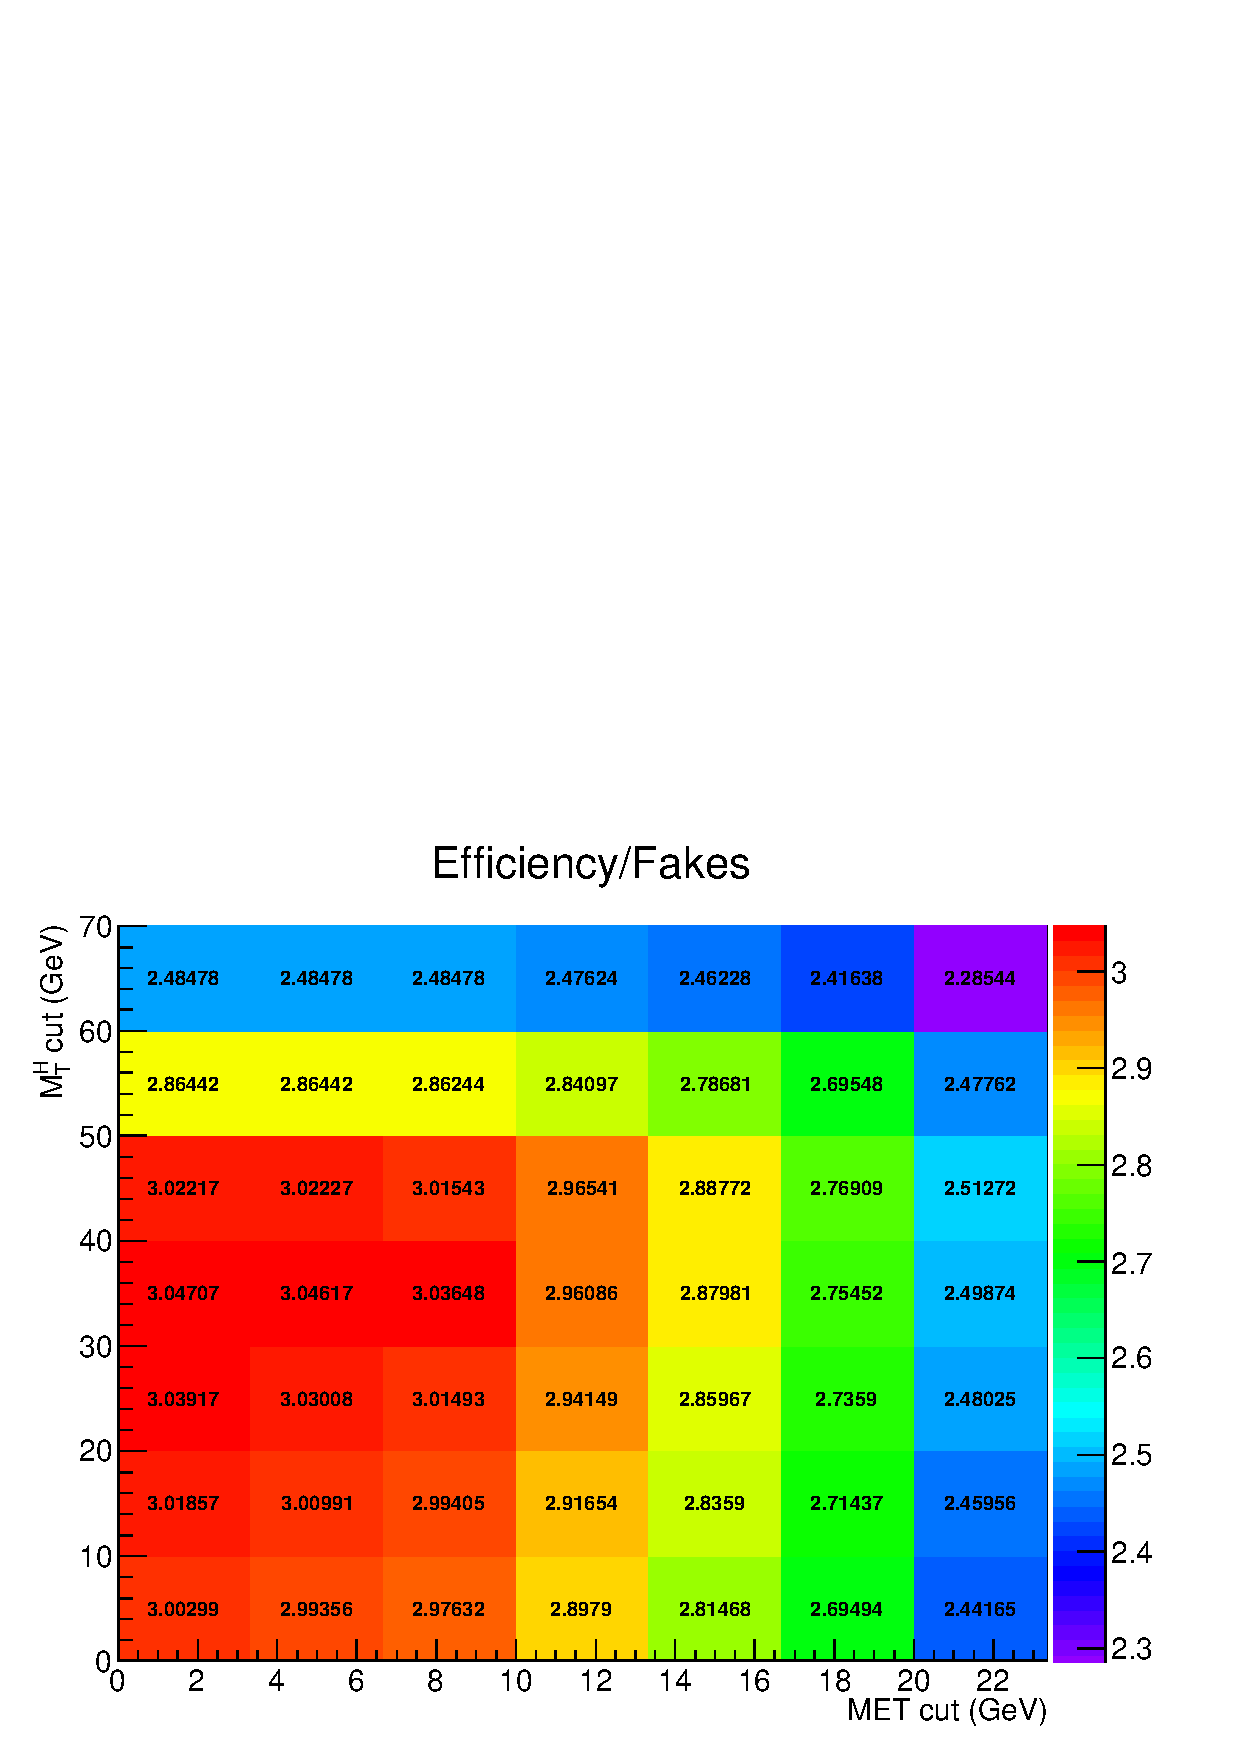
\includegraphics[width=0.5\textwidth]{images/eff_over_fake.pdf}
}
\subfigure{
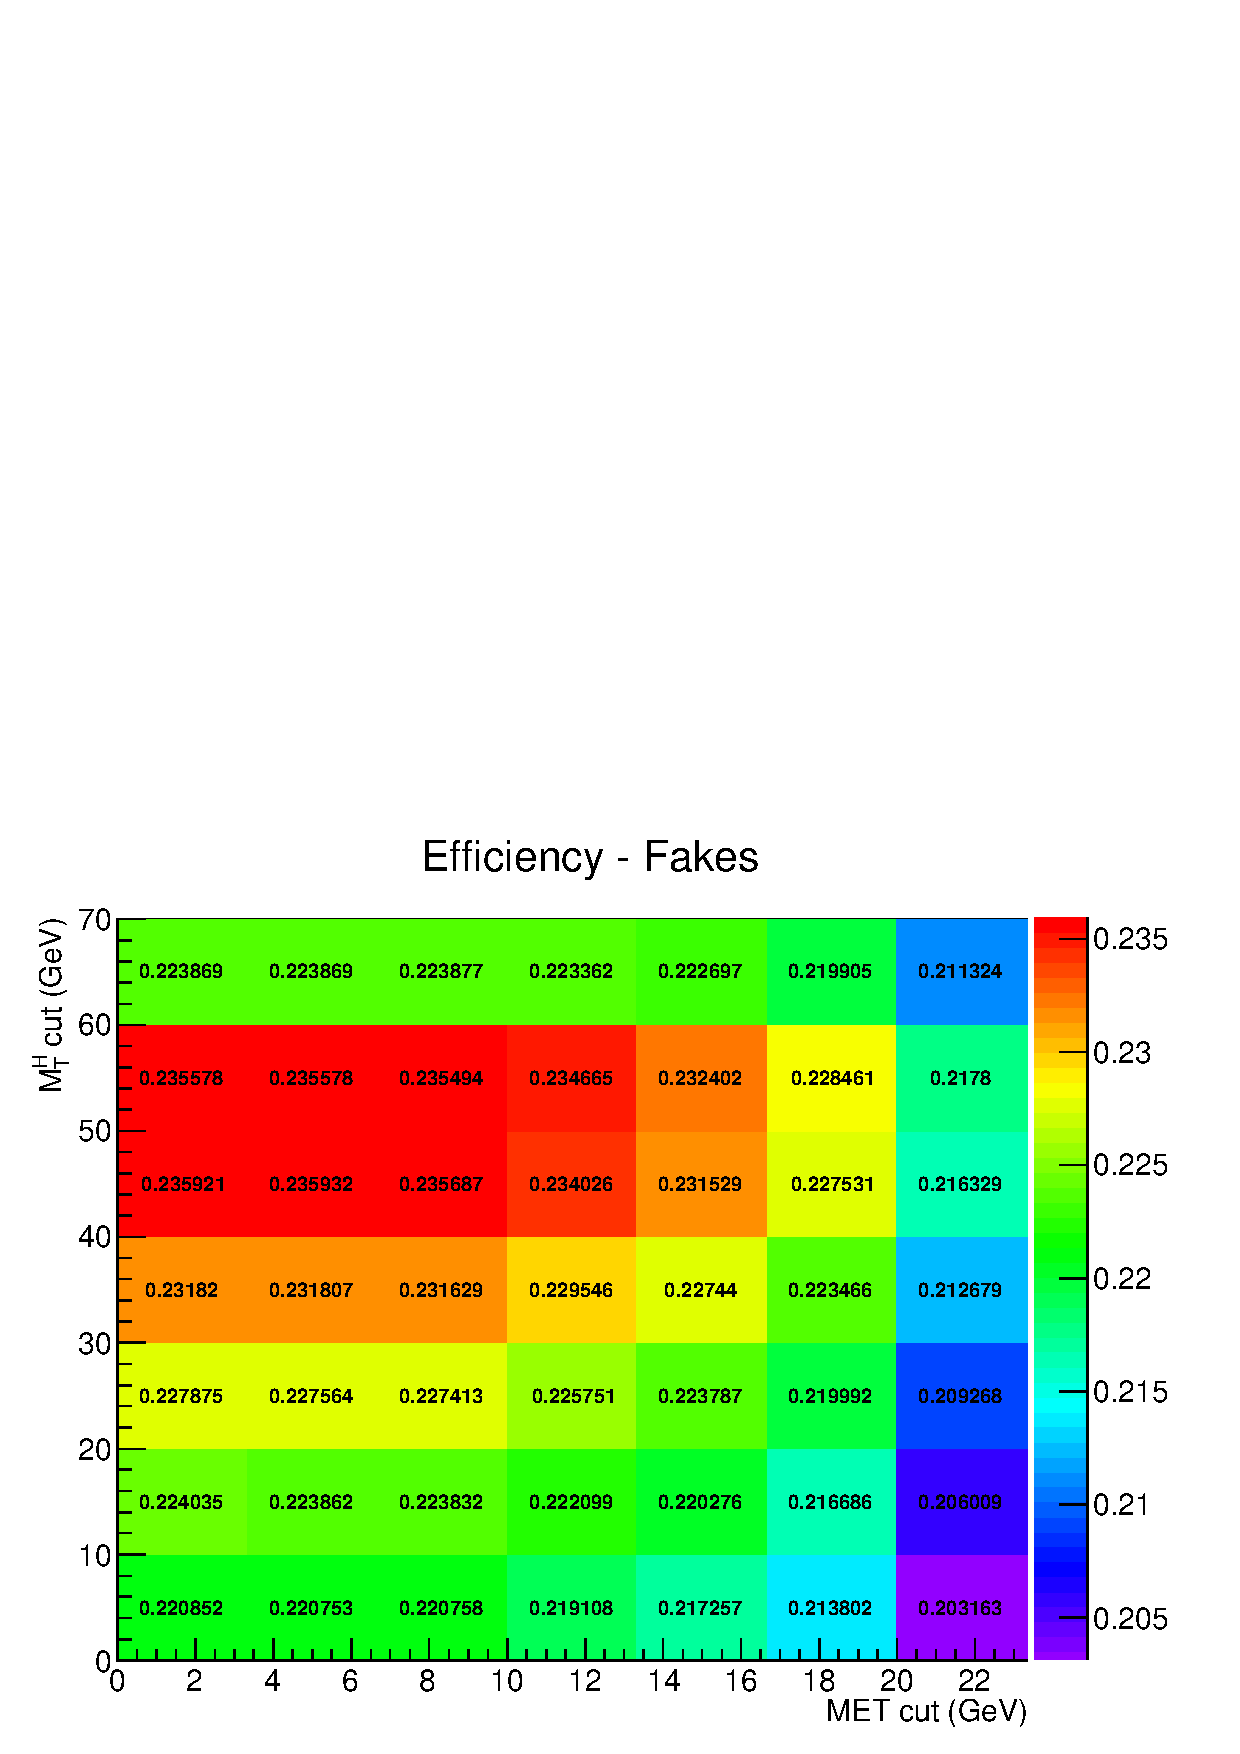
\includegraphics[width=0.5\textwidth]{images/eff-fakes.pdf}
}\\
\subfigure{
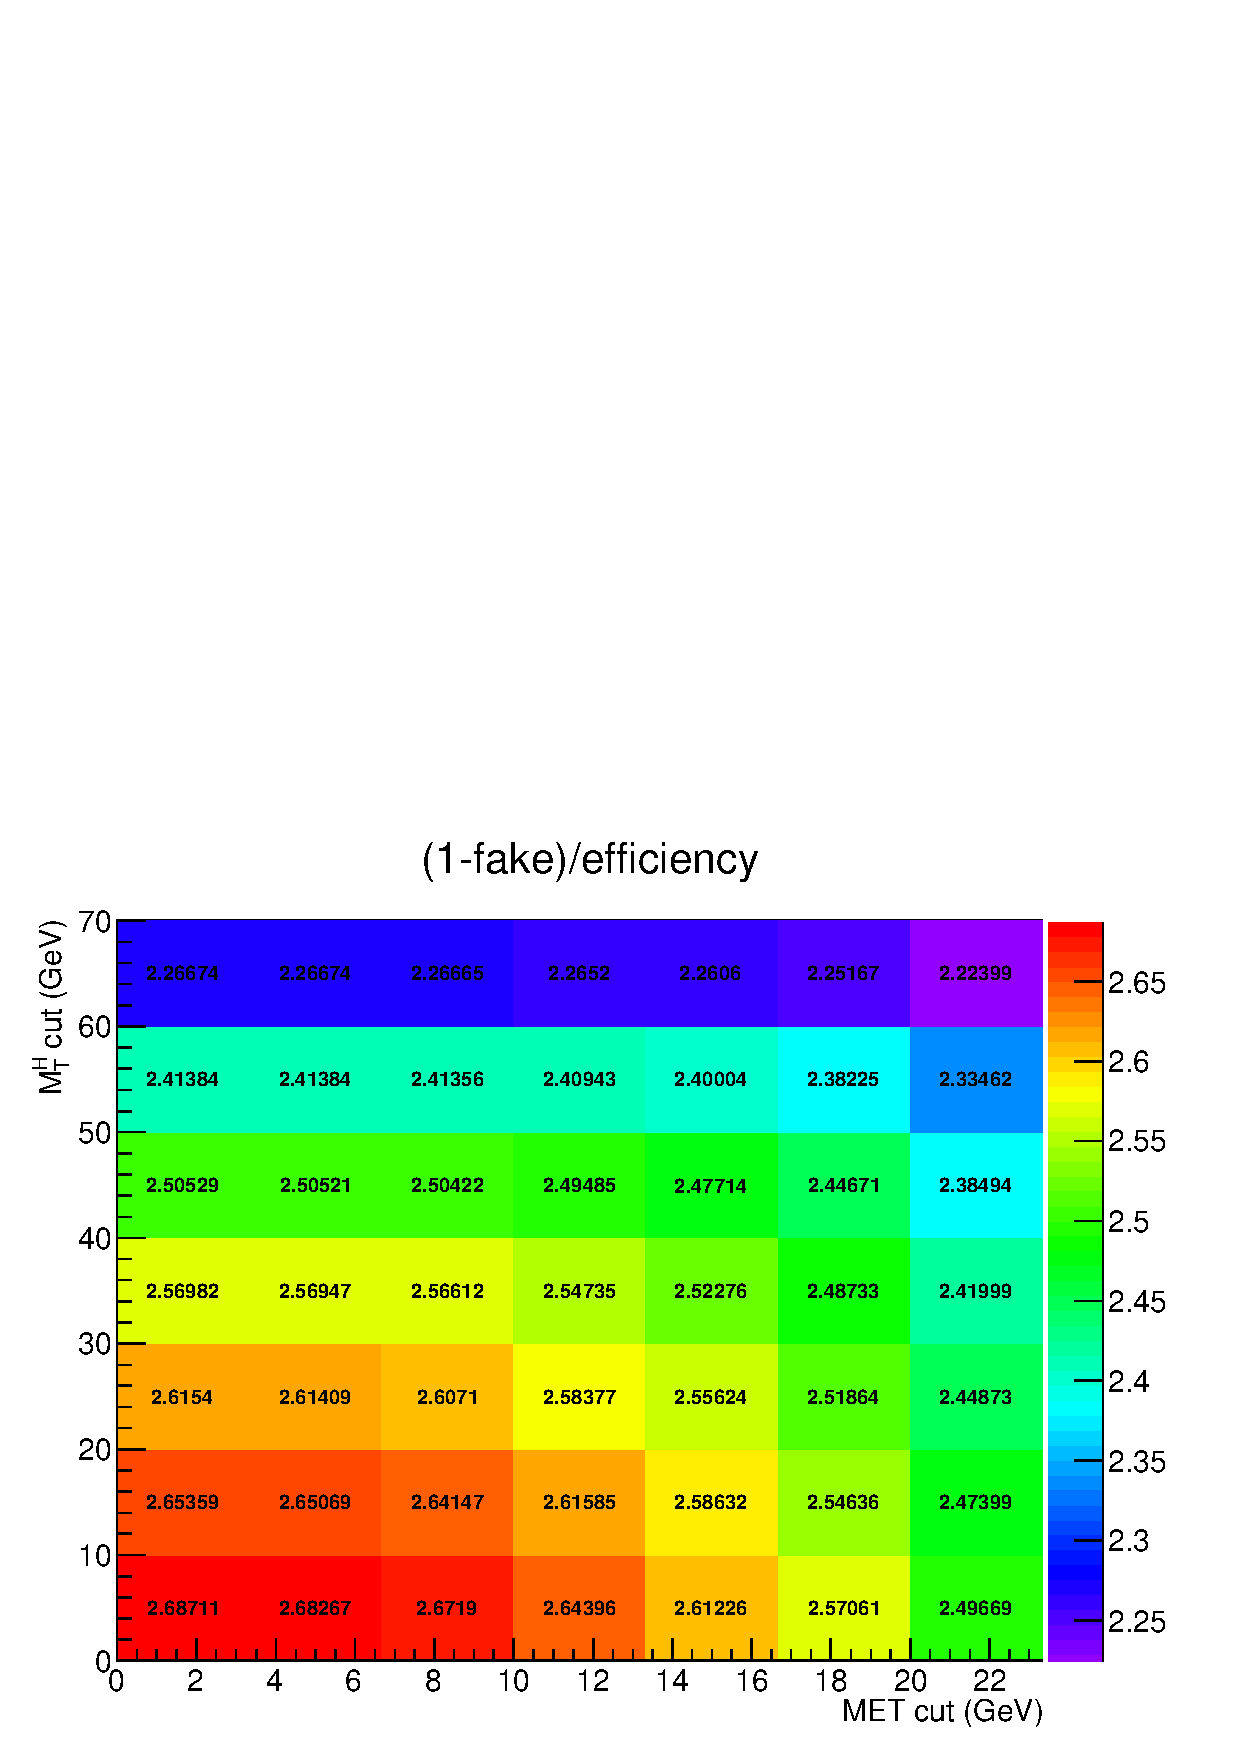
\includegraphics[width=0.5\textwidth]{images/1-fake_over_eff.pdf}
}
\caption{Different figures of merit as a function of \MET and \mt cuts in the fiducial region.}\label{fig:fig_merit_nom}
\end{figure}

Following the same criterion, similar plots as above have been obtained for an alternative model, given by varying up the ggH/VBF ratio within the experimental uncertainties. The results, shown in Fig.~\ref{fig:eff_fake_up} and Fig.~\ref{fig:fig_merit_up}, show a similar trend with respect to the model with nominal ggH/VBF ratio.

\begin{figure}[htb]
\centering
\subfigure{
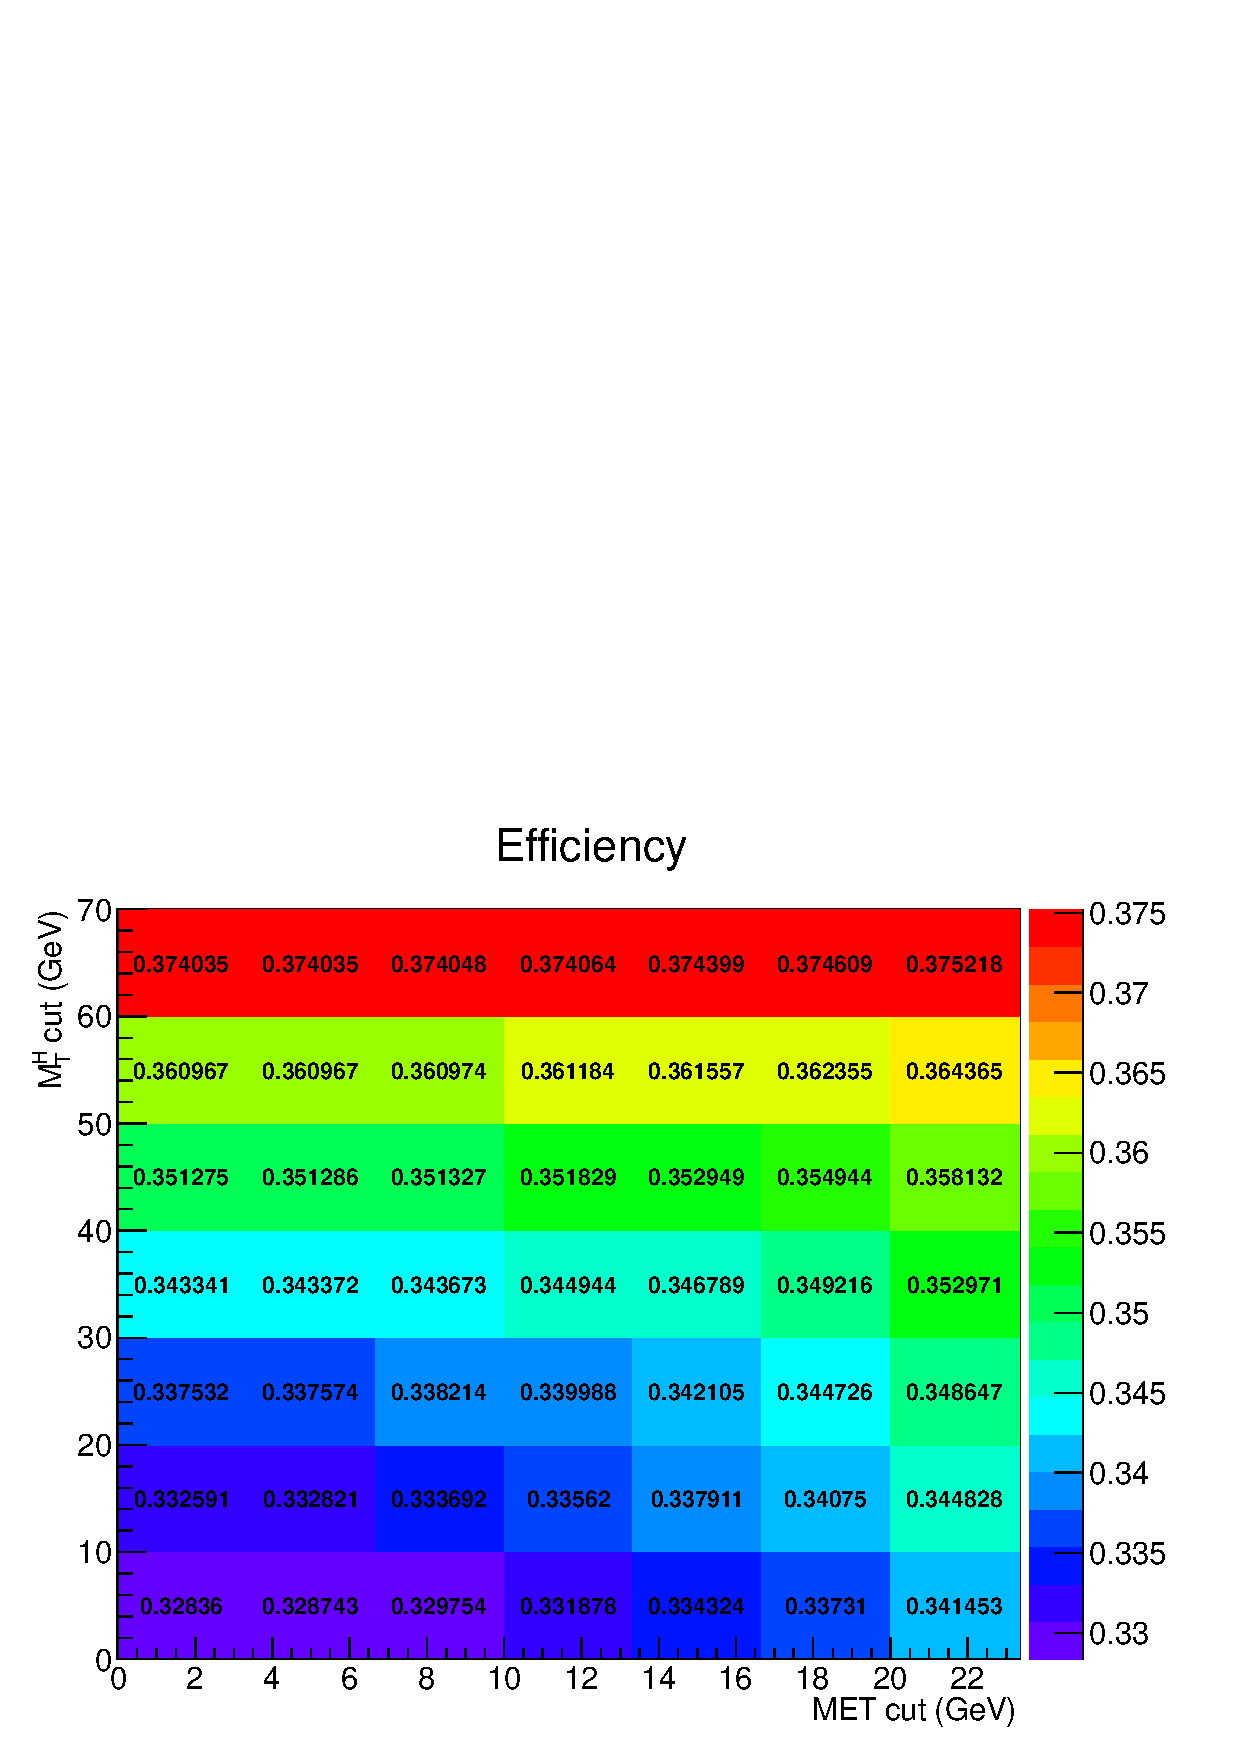
\includegraphics[width=0.5\textwidth]{images/met_mth_eff_UP.pdf}
}
\subfigure{
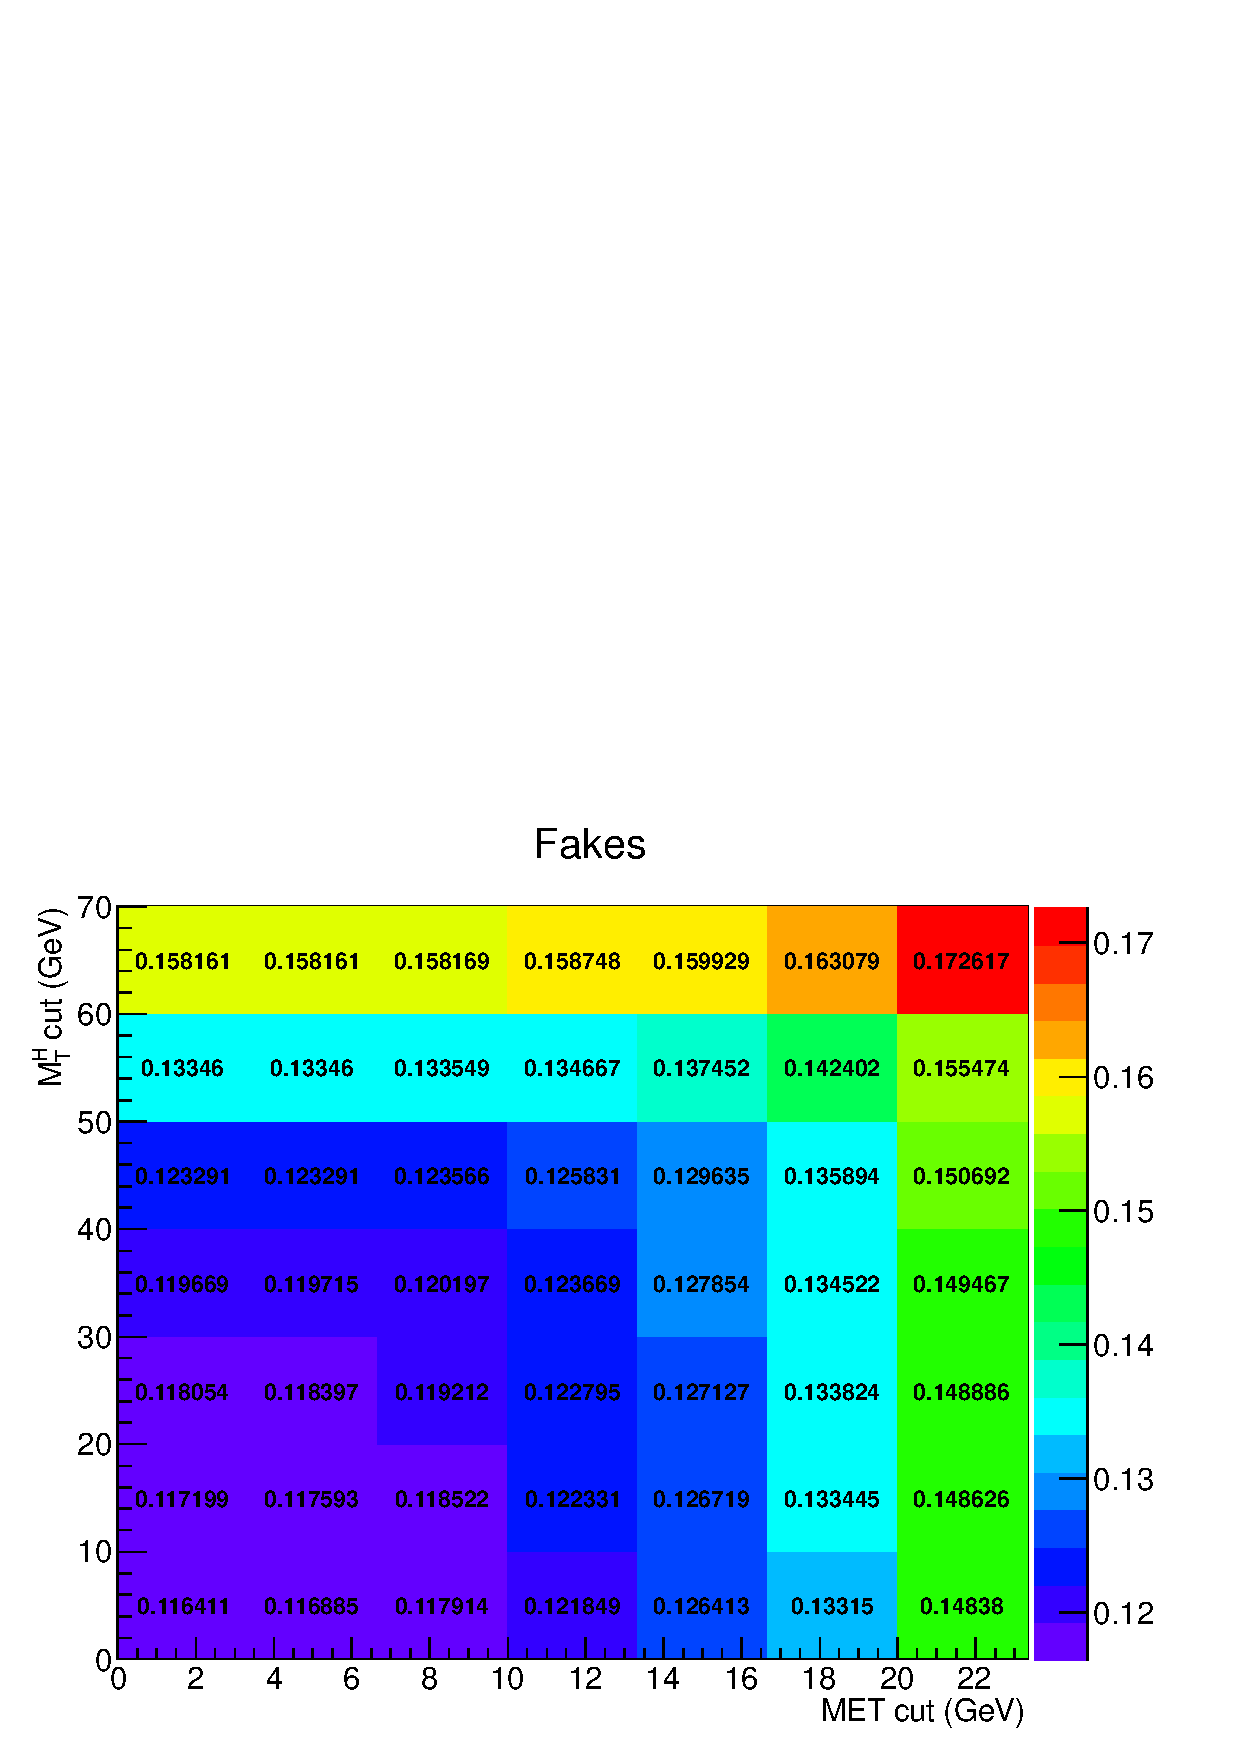
\includegraphics[width=0.5\textwidth]{images/met_mth_fake_UP.pdf}
}
\caption{Efficiency and fake rate as a function of \MET and \mt cuts in the fiducial region, for the alternative model with an up variation of the ggH/VBF ratio.}\label{fig:eff_fake_up}
\end{figure}

\begin{figure}[htb]
\centering
\subfigure{
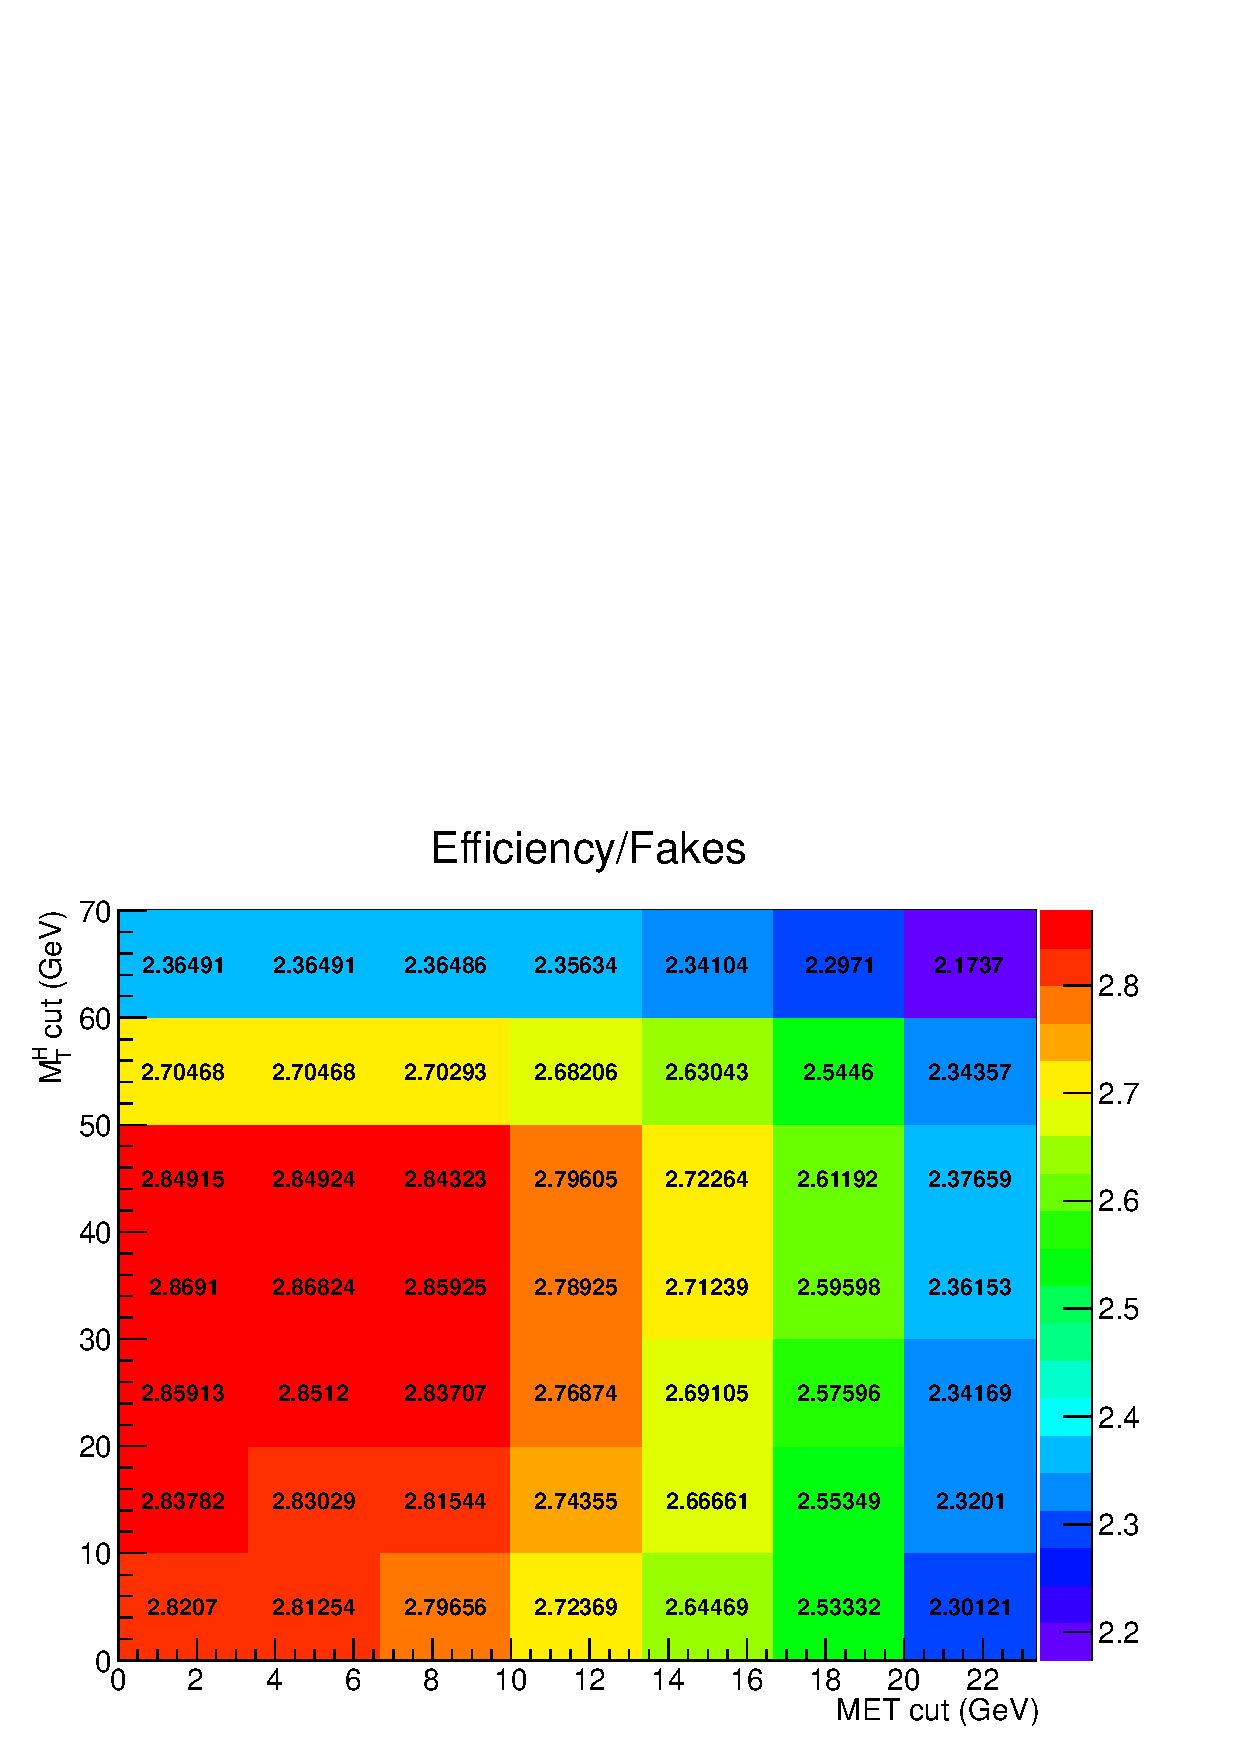
\includegraphics[width=0.5\textwidth]{images/eff_over_fake_UP.pdf}
}
\subfigure{
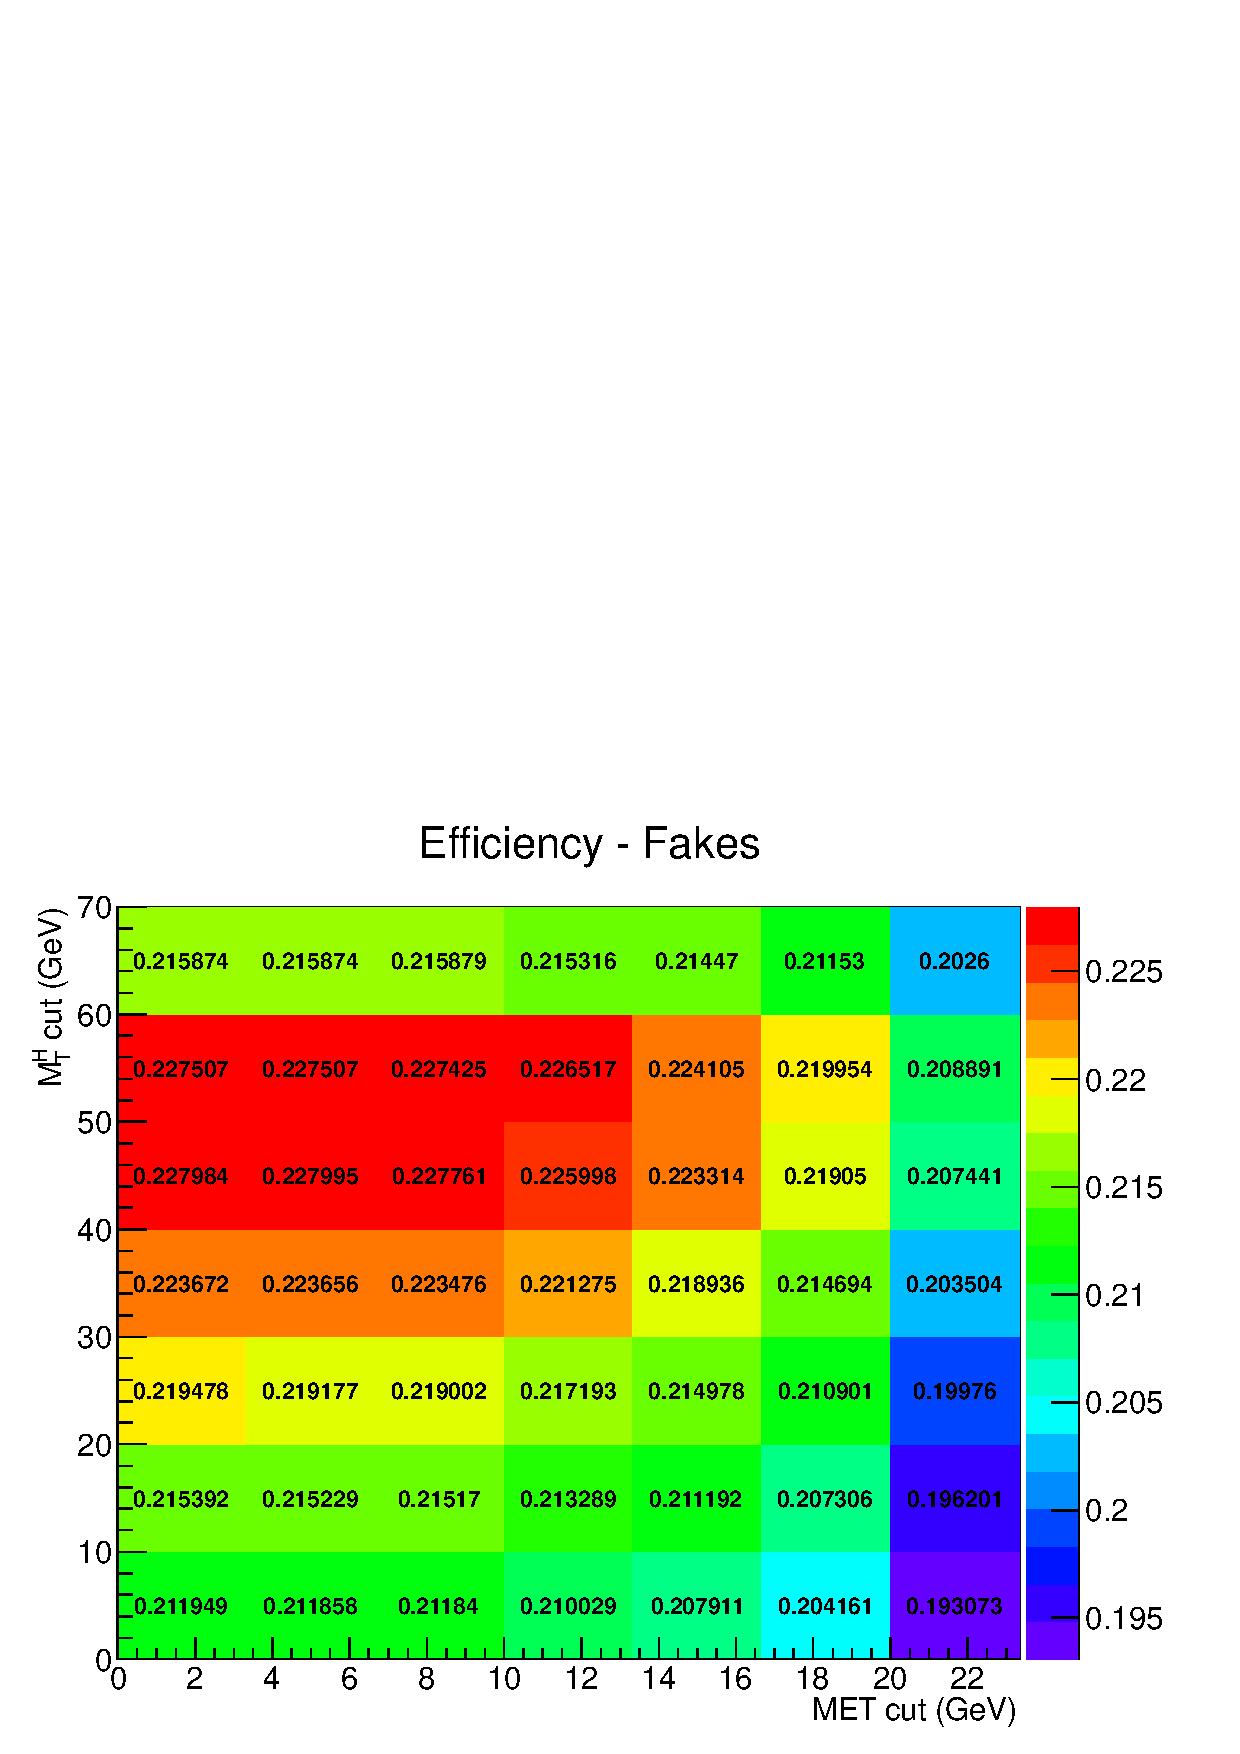
\includegraphics[width=0.5\textwidth]{images/eff-fakes_UP.pdf}
}\\
\subfigure{
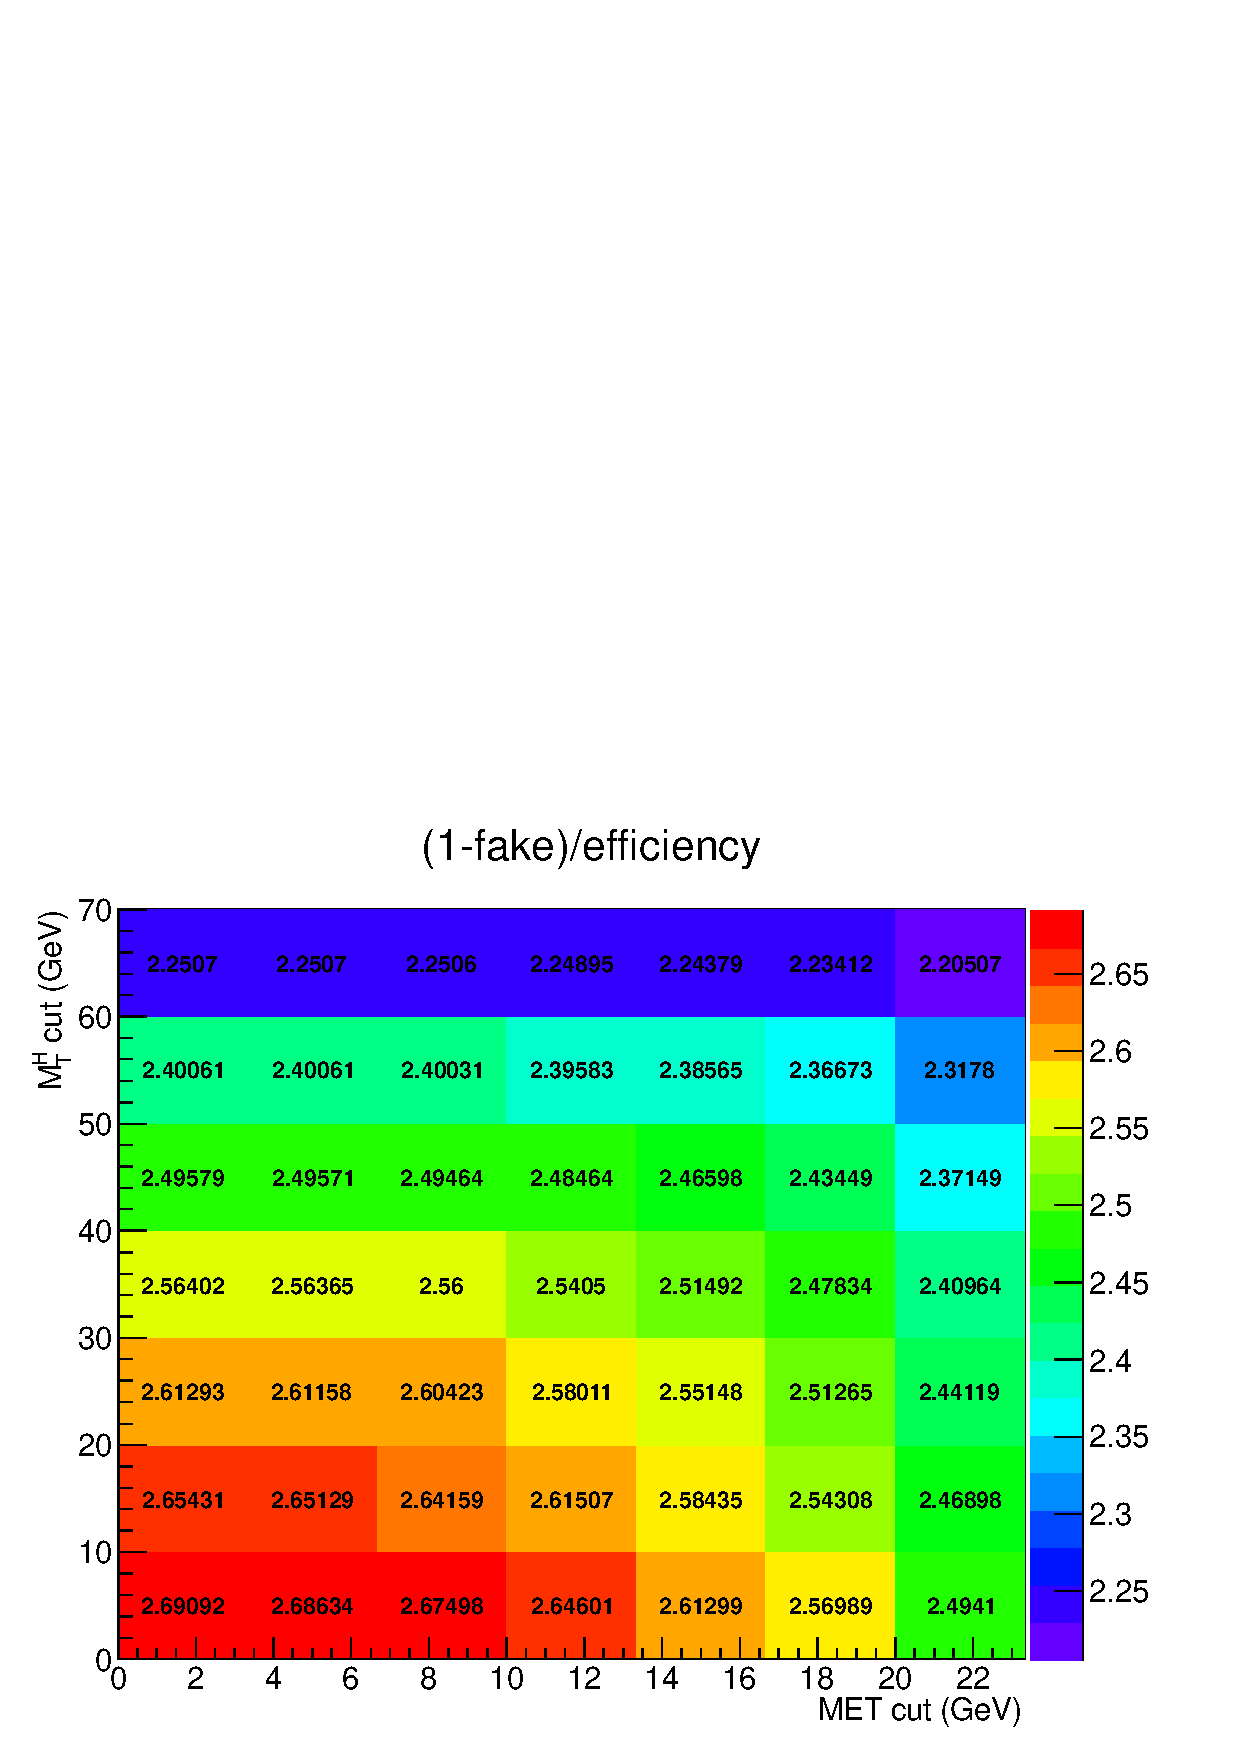
\includegraphics[width=0.5\textwidth]{images/1-fake_over_eff_UP.pdf}
}
\caption{Different figures of merit as a function of \MET and \mt cuts in the fiducial region, for the alternative model with an up variation of the ggH/VBF ratio.}\label{fig:fig_merit_up}
\end{figure}

